\documentclass{standalone}
\usepackage{tikz}
\usetikzlibrary{patterns, positioning}

\begin{document}
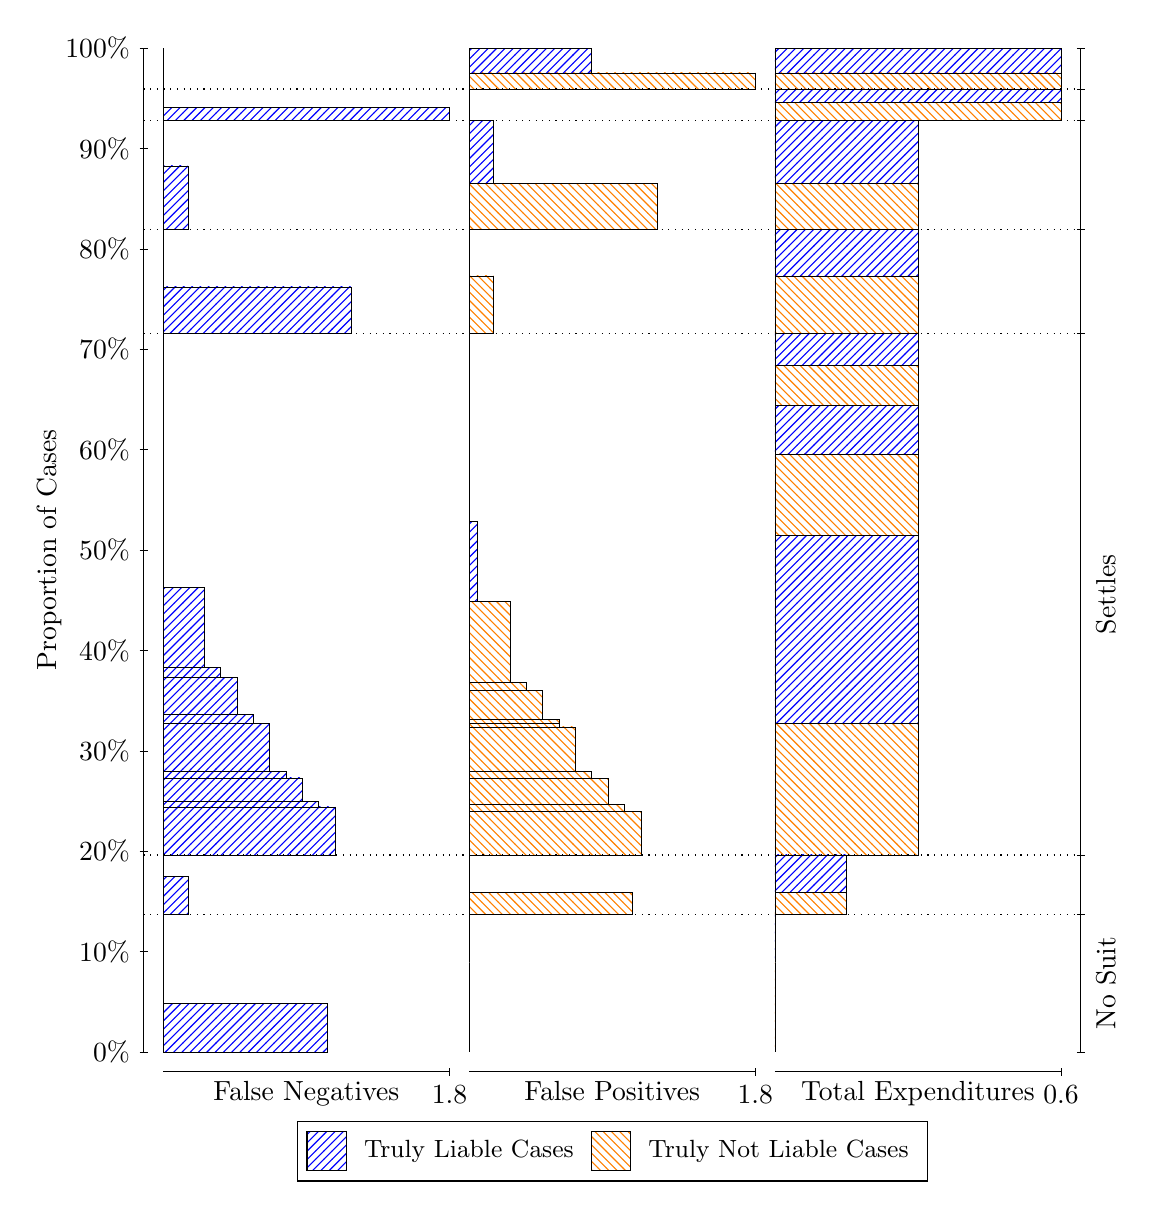
\begin{tikzpicture}
\draw[black, very thin] (1.5,1.75) -- (1.5,14.5);
\node[rotate=90, anchor=center] at (0.3, 8.125) {Proportion of Cases};
\draw[black, very thin] (1.45,1.75) -- (1.55,1.75);
\node[anchor=east] at (1.45, 1.75) {0\%};
\draw[black, very thin] (1.45,3.025) -- (1.55,3.025);
\node[anchor=east] at (1.45, 3.025) {10\%};
\draw[black, very thin] (1.45,4.3) -- (1.55,4.3);
\node[anchor=east] at (1.45, 4.3) {20\%};
\draw[black, very thin] (1.45,5.575) -- (1.55,5.575);
\node[anchor=east] at (1.45, 5.575) {30\%};
\draw[black, very thin] (1.45,6.85) -- (1.55,6.85);
\node[anchor=east] at (1.45, 6.85) {40\%};
\draw[black, very thin] (1.45,8.125) -- (1.55,8.125);
\node[anchor=east] at (1.45, 8.125) {50\%};
\draw[black, very thin] (1.45,9.4) -- (1.55,9.4);
\node[anchor=east] at (1.45, 9.4) {60\%};
\draw[black, very thin] (1.45,10.675) -- (1.55,10.675);
\node[anchor=east] at (1.45, 10.675) {70\%};
\draw[black, very thin] (1.45,11.95) -- (1.55,11.95);
\node[anchor=east] at (1.45, 11.95) {80\%};
\draw[black, very thin] (1.45,13.225) -- (1.55,13.225);
\node[anchor=east] at (1.45, 13.225) {90\%};
\draw[black, very thin] (1.45,14.5) -- (1.55,14.5);
\node[anchor=east] at (1.45, 14.5) {100\%};

\draw[black, very thin] (13.4,1.75) -- (13.4,14.5);
\draw[black, very thin] (13.35,1.75) -- (13.45,1.75);
\node[anchor=west] at (13.35, 1.75) {};
\draw[black, very thin] (13.35,3.5004) -- (13.45,3.5004);
\node[anchor=west] at (13.35, 3.5004) {};
\draw[black, very thin] (13.35,4.2521) -- (13.45,4.2521);
\node[anchor=west] at (13.35, 4.2521) {};
\draw[black, very thin] (13.35,10.874) -- (13.45,10.874);
\node[anchor=west] at (13.35, 10.874) {};
\draw[black, very thin] (13.35,12.201) -- (13.45,12.201);
\node[anchor=west] at (13.35, 12.201) {};
\draw[black, very thin] (13.35,13.58) -- (13.45,13.58);
\node[anchor=west] at (13.35, 13.58) {};
\draw[black, very thin] (13.35,13.98) -- (13.45,13.98);
\node[anchor=west] at (13.35, 13.98) {};
\draw[black, very thin] (13.35,14.5) -- (13.45,14.5);
\node[anchor=west] at (13.35, 14.5) {};

\draw[black, very thin, pattern color=blue, pattern=north east lines] (1.75,1.75) rectangle (3.8262,2.3669);
\draw[black, very thin, pattern color=orange, pattern=north west lines] (1.75,2.3669) rectangle (1.75,3.5004);
\draw[black, very thin, pattern color=blue, pattern=north east lines] (1.75,3.5004) rectangle (2.0614,3.9791);
\draw[black, very thin, pattern color=orange, pattern=north west lines] (1.75,3.9791) rectangle (1.75,4.2521);
\draw[black, very thin, pattern color=blue, pattern=north east lines] (1.75,4.2521) rectangle (3.93,4.8639);
\draw[black, very thin, pattern color=blue, pattern=north east lines] (1.75,4.8639) rectangle (3.7224,4.9304);
\draw[black, very thin, pattern color=blue, pattern=north east lines] (1.75,4.9304) rectangle (3.5148,5.2302);
\draw[black, very thin, pattern color=blue, pattern=north east lines] (1.75,5.2302) rectangle (3.3071,5.312);
\draw[black, very thin, pattern color=blue, pattern=north east lines] (1.75,5.312) rectangle (3.0995,5.9218);
\draw[black, very thin, pattern color=blue, pattern=north east lines] (1.75,5.9218) rectangle (2.8919,6.0346);
\draw[black, very thin, pattern color=blue, pattern=north east lines] (1.75,6.0346) rectangle (2.6843,6.5099);
\draw[black, very thin, pattern color=blue, pattern=north east lines] (1.75,6.5099) rectangle (2.4767,6.6383);
\draw[black, very thin, pattern color=blue, pattern=north east lines] (1.75,6.6383) rectangle (2.269,7.6524);
\draw[black, very thin, pattern color=orange, pattern=north west lines] (1.75,7.6524) rectangle (1.75,10.874);
\draw[black, very thin, pattern color=blue, pattern=north east lines] (1.75,10.874) rectangle (4.1376,11.467);
\draw[black, very thin, pattern color=orange, pattern=north west lines] (1.75,11.467) rectangle (1.75,12.201);
\draw[black, very thin, pattern color=blue, pattern=north east lines] (1.75,12.201) rectangle (2.0614,13.003);
\draw[black, very thin, pattern color=orange, pattern=north west lines] (1.75,13.003) rectangle (1.75,13.58);
\draw[black, very thin, pattern color=blue, pattern=north east lines] (1.75,13.58) rectangle (5.3833,13.747);
\draw[black, very thin, pattern color=orange, pattern=north west lines] (1.75,13.747) rectangle (1.75,13.98);
\draw[black, very thin, pattern color=orange, pattern=north west lines] (1.75,13.98) rectangle (1.75,14.185);
\draw[black, very thin, pattern color=blue, pattern=north east lines] (1.75,14.185) rectangle (1.75,14.5);
\draw[black, very thin, pattern color=orange, pattern=north west lines] (5.6333,1.75) rectangle (5.6333,2.8835);
\draw[black, very thin, pattern color=blue, pattern=north east lines] (5.6333,2.8835) rectangle (5.6333,3.5004);
\draw[black, very thin, pattern color=orange, pattern=north west lines] (5.6333,3.5004) rectangle (7.7095,3.7735);
\draw[black, very thin, pattern color=blue, pattern=north east lines] (5.6333,3.7735) rectangle (5.6333,4.2521);
\draw[black, very thin, pattern color=orange, pattern=north west lines] (5.6333,4.2521) rectangle (7.8133,4.8102);
\draw[black, very thin, pattern color=orange, pattern=north west lines] (5.6333,4.8102) rectangle (7.6057,4.8925);
\draw[black, very thin, pattern color=orange, pattern=north west lines] (5.6333,4.8925) rectangle (7.3981,5.226);
\draw[black, very thin, pattern color=orange, pattern=north west lines] (5.6333,5.226) rectangle (7.1905,5.3136);
\draw[black, very thin, pattern color=orange, pattern=north west lines] (5.6333,5.3136) rectangle (6.9829,5.8789);
\draw[black, very thin, pattern color=orange, pattern=north west lines] (5.6333,5.8789) rectangle (6.7752,5.9271);
\draw[black, very thin, pattern color=orange, pattern=north west lines] (5.6333,5.9271) rectangle (6.7752,5.9709);
\draw[black, very thin, pattern color=orange, pattern=north west lines] (5.6333,5.9709) rectangle (6.5676,6.3423);
\draw[black, very thin, pattern color=orange, pattern=north west lines] (5.6333,6.3423) rectangle (6.36,6.4396);
\draw[black, very thin, pattern color=orange, pattern=north west lines] (5.6333,6.4396) rectangle (6.1524,7.4734);
\draw[black, very thin, pattern color=blue, pattern=north east lines] (5.6333,7.4734) rectangle (5.7371,8.4874);
\draw[black, very thin, pattern color=blue, pattern=north east lines] (5.6333,8.4874) rectangle (5.6333,10.874);
\draw[black, very thin, pattern color=orange, pattern=north west lines] (5.6333,10.874) rectangle (5.9448,11.607);
\draw[black, very thin, pattern color=blue, pattern=north east lines] (5.6333,11.607) rectangle (5.6333,12.201);
\draw[black, very thin, pattern color=orange, pattern=north west lines] (5.6333,12.201) rectangle (8.021,12.777);
\draw[black, very thin, pattern color=blue, pattern=north east lines] (5.6333,12.777) rectangle (5.9448,13.58);
\draw[black, very thin, pattern color=orange, pattern=north west lines] (5.6333,13.58) rectangle (5.6333,13.813);
\draw[black, very thin, pattern color=blue, pattern=north east lines] (5.6333,13.813) rectangle (5.6333,13.98);
\draw[black, very thin, pattern color=orange, pattern=north west lines] (5.6333,13.98) rectangle (9.2667,14.185);
\draw[black, very thin, pattern color=blue, pattern=north east lines] (5.6333,14.185) rectangle (7.1905,14.5);
\draw[black, very thin, pattern color=orange, pattern=north west lines] (9.5167,1.75) rectangle (9.5167,2.8835);
\draw[black, very thin, pattern color=blue, pattern=north east lines] (9.5167,2.8835) rectangle (9.5167,3.5004);
\draw[black, very thin, pattern color=orange, pattern=north west lines] (9.5167,3.5004) rectangle (10.425,3.7735);
\draw[black, very thin, pattern color=blue, pattern=north east lines] (9.5167,3.7735) rectangle (10.425,4.2521);
\draw[black, very thin, pattern color=orange, pattern=north west lines] (9.5167,4.2521) rectangle (11.333,5.9271);
\draw[black, very thin, pattern color=blue, pattern=north east lines] (9.5167,5.9271) rectangle (11.333,8.3123);
\draw[black, very thin, pattern color=orange, pattern=north west lines] (9.5167,8.3123) rectangle (11.333,9.3461);
\draw[black, very thin, pattern color=blue, pattern=north east lines] (9.5167,9.3461) rectangle (11.333,9.9579);
\draw[black, very thin, pattern color=orange, pattern=north west lines] (9.5167,9.9579) rectangle (11.333,10.47);
\draw[black, very thin, pattern color=blue, pattern=north east lines] (9.5167,10.47) rectangle (11.333,10.874);
\draw[black, very thin, pattern color=orange, pattern=north west lines] (9.5167,10.874) rectangle (11.333,11.607);
\draw[black, very thin, pattern color=blue, pattern=north east lines] (9.5167,11.607) rectangle (11.333,12.201);
\draw[black, very thin, pattern color=orange, pattern=north west lines] (9.5167,12.201) rectangle (11.333,12.777);
\draw[black, very thin, pattern color=blue, pattern=north east lines] (9.5167,12.777) rectangle (11.333,13.58);
\draw[black, very thin, pattern color=orange, pattern=north west lines] (9.5167,13.58) rectangle (13.15,13.813);
\draw[black, very thin, pattern color=blue, pattern=north east lines] (9.5167,13.813) rectangle (13.15,13.98);
\draw[black, very thin, pattern color=orange, pattern=north west lines] (9.5167,13.98) rectangle (13.15,14.185);
\draw[black, very thin, pattern color=blue, pattern=north east lines] (9.5167,14.185) rectangle (13.15,14.5);
\draw[black, dotted] (1.5,3.5004) -- (13.4,3.5004);
\draw[black, dotted] (1.5,4.2521) -- (13.4,4.2521);
\draw[black, dotted] (1.5,10.874) -- (13.4,10.874);
\draw[black, dotted] (1.5,12.201) -- (13.4,12.201);
\draw[black, dotted] (1.5,13.58) -- (13.4,13.58);
\draw[black, dotted] (1.5,13.98) -- (13.4,13.98);
\draw[black, very thin] (1.75,1.5) -- (5.3833,1.5);
\node[anchor=north] at (3.5667, 1.5) {False Negatives};
\draw[black, very thin] (5.3833,1.45) -- (5.3833,1.55);
\node[anchor=north] at (5.3833, 1.45) {1.8};

\draw[black, very thin] (5.6333,1.5) -- (9.2667,1.5);
\node[anchor=north] at (7.45, 1.5) {False Positives};
\draw[black, very thin] (9.2667,1.45) -- (9.2667,1.55);
\node[anchor=north] at (9.2667, 1.45) {1.8};

\draw[black, very thin] (9.5167,1.5) -- (13.15,1.5);
\node[anchor=north] at (11.333, 1.5) {Total Expenditures};
\draw[black, very thin] (13.15,1.45) -- (13.15,1.55);
\node[anchor=north] at (13.15, 1.45) {0.6};

\node[black, centered, rotate=90] at (13.72, 2.6252) {No Suit};

\node[black, centered, rotate=90] at (13.72, 7.5629) {Settles};





\draw (7.449999999999999,1.5) node[draw=none] (baseCoordinate) {};
\begin{scope}[align=center]
        \matrix[scale=0.5, draw=black, below=0.5cm of baseCoordinate, nodes={draw}, column sep=0.1cm]{
            \node[rectangle, draw, minimum width=0.5cm, minimum height=0.5cm, pattern=north east lines, pattern color=blue] {}; &
            \node[draw=none, font=\small] (B) {Truly Liable Cases}; &
            \node[rectangle, draw, minimum width=0.5cm, minimum height=0.5cm, pattern=north west lines, pattern color=orange] {}; &
            \node[draw=none, font=\small] (B) {Truly Not Liable Cases}; \\
            };
\end{scope}

\end{tikzpicture}
\end{document}